\section{Experiments}
\label{sec:exp}

This section presents the results of our experiments on the finite-field multipliers.
We compare an implementation of~\autoref{sec:theory}  
against the incremental SAT based approach presented in~\cite{fujita:2015}.
We have implemented the approach presented in~\cite{fujita:2015} using
Python with PICOSAT as the underlying SAT solver. The experiments were performed on a 4.0GHz 
Intel(R) $\text{Core}^{\text{TM}}$ i7-6700K Quad-Core CPU with 32 GB of RAM.
\subsection{Mastrovito Multipliers}
Modular multiplication is an important operation used in cryptography. 
A Mastrovito multiplier architecture can be used for performing this computation.
Mastrovito multipliers compute $Z = A\times B \pmod{P(x)}$ where $P(x)$ is a given primitive polynomial for the datapath size
$k$. The product $A \times B$ is computed using an array multiplier architecture, and then the result is reduced modulo $P(x)$.
% The following example demonstrates the Mastrovito multiplier computation~\cite{lv:tcad2013}.
%take $\{A,B\} =
%\{a_0,a_1,\dots,a_{k-1},b_0,b_1,\dots,b_{k-1}\}$ as $k$-bit inputs and
%produce $Z = \{z_0,z_1,\dots,z_{k-1}\}$ as $k$-bit output. The multiplier
%performs $Z = A \times B \pmod{P}$, 
%The procedure 
%involves computing the product $S=A\times B$ using an array multiplier
%and then reducing it $\pmod{P}$ to obtain $Z$. We perform experiments
%on \textit{flattened} netlists of these circuits.  
% \begin{Example}
% \label{exp1}
% {\it 
% Consider the field $\mathbb{F}_{2^4}$. Let the inputs be:
% $A=a_0+a_1\cdot \alpha+a_2\cdot \alpha^2+a_3\cdot \alpha^3$ and
% $B=b_0+b_1\cdot \alpha+b_2\cdot \alpha^2+b_3\cdot \alpha^3$, and 
%  the irreducible polynomial be $P(x)=x^4+x^3+1$. 
%  % We have to perform the multiplication $Z =A\times B \pmod{ P(x) }$. 
%  The coefficients of $A = \{a_0, \dots, a_3\}, B = \{b_0, \dots, b_3\}$ are in
% $\mathbb{F}_2 = \{0, 1\}$. First, we perform the multiplication as:
% %\vspace{-0.2in}
% \vspace{0.05in}
% {\small
% {\begin{tabular}{c c c c c c c c}
% %\vspace{-0.2in}
%   &   &   & $a_3$ & $a_2$ & $a_1$ & $a_0$  \\ 
%  $\times$&   &   & $b_3$ & $b_2$ & $b_1$ & $b_0$  \\ 
%  \hline
%  &   &   & $a_3\cdot b_0$ & $a_2 \cdot b_0$ & $a_1\cdot b_0$ & $a_0\cdot b_0$ \\
%  &  & $a_3\cdot b_1$ & $a_2\cdot b_1$ & $a_1 \cdot b_1$ & $a_0\cdot b_1$ &   \\
%  & $a_3\cdot b_2$ & $a_2\cdot b_2$ & $a_1\cdot b_2$ & $a_0\cdot b_2$ &  &   \\
%  $a_3\cdot b_3$ & $a_2\cdot b_3$ & $a_1\cdot b_3$ & $a_0\cdot b_3$ &  &  &   \\
%  \hline
%  $s_6$& $s_5$  & $s_4$  & $s_3$ & $s_2$  & $s_1$   & $s_0$ 
% % \vspace{-0.2in}
% \end{tabular}}
% }
% \vspace{0.05in}
% The result $Sum = s_0+s_1\cdot \alpha + s_2\cdot \alpha^2 + s_3\cdot
% \alpha^3 + s_4\cdot \alpha^4 + s_5\cdot \alpha^5 + s_6\cdot \alpha^6$,
% where, $s_0  =  a_0\cdot b_0, ~~s_1  =  a_0\cdot b_1 + a_1\cdot b_0,
% ~~s_2 = a_0\cdot b_2 + a_1\cdot b_1 + a_2\cdot b_0$, and so on. Here
% the multiply ``$\cdot$'' and add ``$+$'' operations are performed
% modulo 2, and hence implemented in a circuit using AND and XOR
% gates. As the coefficients are always reduced modulo $p =
% 2$, there are no carry-chains
% in the design. Next, the result is reduced modulo the primitive
% polynomial $P(x) = x^4 + x^3 + 1$, as:
% % where the final output of the circuit is denoted by $G(x)  = g_3x^3
% % + g_2x^2 +g_1x + g_0$.  
% \vspace{0.05in}
% {\small
% {\begin{tabular}{|c c c c | l }
%   $s_3$   &$s_2$    &$s_1$   &$s_0$   &   \\
%  \hline
%  $s_4$    &$0$    &$0$   &$s_4$   &$s_4\cdot \alpha^4 \pmod{P(\alpha)} = s_4 \cdot (\alpha^3 + 1)$\\
%  $s_5$    &$0$    &$s_5$   &$s_5$     &$s_5\cdot \alpha^5 \pmod{P(\alpha)} = s_5\cdot (\alpha^3+ \alpha + 1)$\\
%  $s_6$    &$s_6$    &$s_6$   &$s_6$     &$s_6\cdot \alpha^6 \pmod{ P(\alpha)} = s_6\cdot( \alpha^3 + \alpha^2 + \alpha + 1)$\\
%  \hline
%  $z_3$    &$z_2$    &$z_1$   &$z_0$   &
%  \end{tabular}\par}
% }
% \vspace{0.05in}
% The final output of the circuit is: $Z = z_0 + z_1 \alpha + z_2
% \alpha^2 + z_3 \alpha^3$; where  $z_0=s_0+s_4+s_5+s_6; ~~z_1=s_1+s_5+s_6;
% ~~z_2=s_2+s_6; ~~z_3=s_3+s_4+s_5+s_6$. 
% }
% \end{Example}
\subsection{Montgomery Multipliers}
Exponentiation (repeated multiplication) is often required in cryptosystems.  
For such applications, Montgomery architecture~\cite{acar:1998},~\cite{wu:2002},
% \cite{Barrett:1987} 
~\cite{knezevic:2008} are considered more efficient than Mastrovito multipliers
as they do not require explicit reduction modulo $P(x)$ after each step.
~\autoref{montfig} shows the structure of a Montgomery
multiplier. Each MR block computes $A\cdot B\cdot R^{-1}$, where $R$
is selected as a power of a base ($\alpha^{k}$) and $R^{-1}$ is the multiplicative 
inverse of $R$ in $\mathbb{F}_{2^k}$. As this operation cannot compute $A\cdot B$
directly, we need to pre-compute $A\cdot R$ and $B\cdot R$ as shown in the~\autoref{montfig}. 
We denote the leftmost
two blocks as Block A (upper) and B (lower), the middle block as Block
C and the output block as Block D.
% We have presented results for GBR
%on both \textit{flattened} and \textit{hierarchical} netlists of these
% multipliers. 

\begin{figure}[H]
  \centering
  %\def\svgwidth{340pt}
  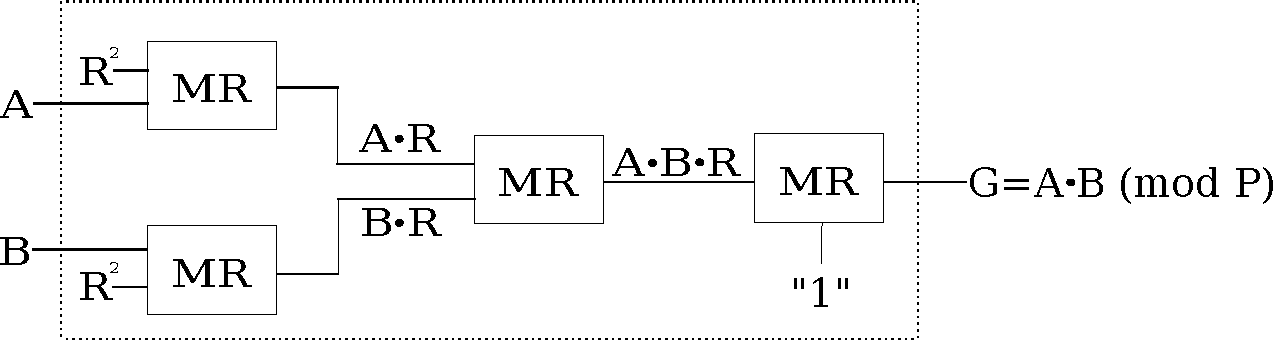
\includegraphics[scale=0.34]{new_mmcircuit-eps-converted-to}
  \caption{Montgomery multiplication.}
  \label{montfig}
  \end{figure}
\vspace{-0.05in}

~\autoref{masusmontspec} presents the execution times when there is an unknown component in the Mastrovito multiplier and Montgomery multiplier is used as the specification. The labels $NO$, $NM$, and $NI$ denote the unknown component placed near output, somewhere in the middle, and near input respectively. While the approach~\cite{fujita:2015} finds a satisfying transformation assignment which can be mapped to a library gate, our approach~\autoref{sec:theory} outputs a function in terms of primary input bits which can be implemented as a single gate or sub-circuit. As shown in the table, our approach shows improvement by several orders of magnitude.

\begin{table}[H]
\centering
\caption{{Resolving Unknown Component in Mastrovito circuit v/s Reference Specification Montgomery}( Time is in seconds); k = Datapath Size of both multipliers, Time-Out = 12 hrs}
\label{masusmontspec}
\begin{tabular}{| c | c | c | c | c | c | c |} \hline
\multirow{2}{*}{\textbf{k}}& \multicolumn{3}{ c |}{\textbf{~\cite{fujita:2015}}}& \multicolumn{3}{ c |}{\textbf{~\autoref{sec:theory}}}\\ \cline{2-7}
&{\it NO}&{\it NM}&{\it NI}&{\it NO}&{\it NM}&{\it NI} \\ \hline
9&33.7&36.8&34.9& 11.1 & 5.4 & 1.4\\ \hline
10&214.3&215&231.4& 48.9 & 29.3 & 4.9\\ \hline
11&1,999.5&1,927&2,090.7& 120.5 & 96.1 & 8.9\\ \hline
12&24,085&23,400& 8,676& 3880.6 & 2140.3 & 243.7\\ \hline
13&TO&TO&TO& 4143 & 2735.9 & 321.6\\ \hline
% 16&TO&TO&TO&  &  & \\ \hline
% 32&TO&TO&TO&  &  & \\ \hline
% 64&TO&TO&TO&  &  & \\ \hline
\end{tabular}
\end{table}